\clearpage\thispagestyle{empty}\SourceLeaf{002}
\vspace*{1cm}
\begin{center}\small
\textbf{CARL FRIEDRICH GAUSS: WORKS}\\[1em]
\textbf{VOLUME III.}
\end{center}
\clearpage

\clearpage\thispagestyle{empty}\SourceLeaf{004}
\vspace*{1cm}
\begin{center}\small
\textbf{CARL FRIEDRICH GAUSS}\\[0.5em]
\textbf{WORKS}\\[1em]
\textbf{THIRD VOLUME}\\[2em]
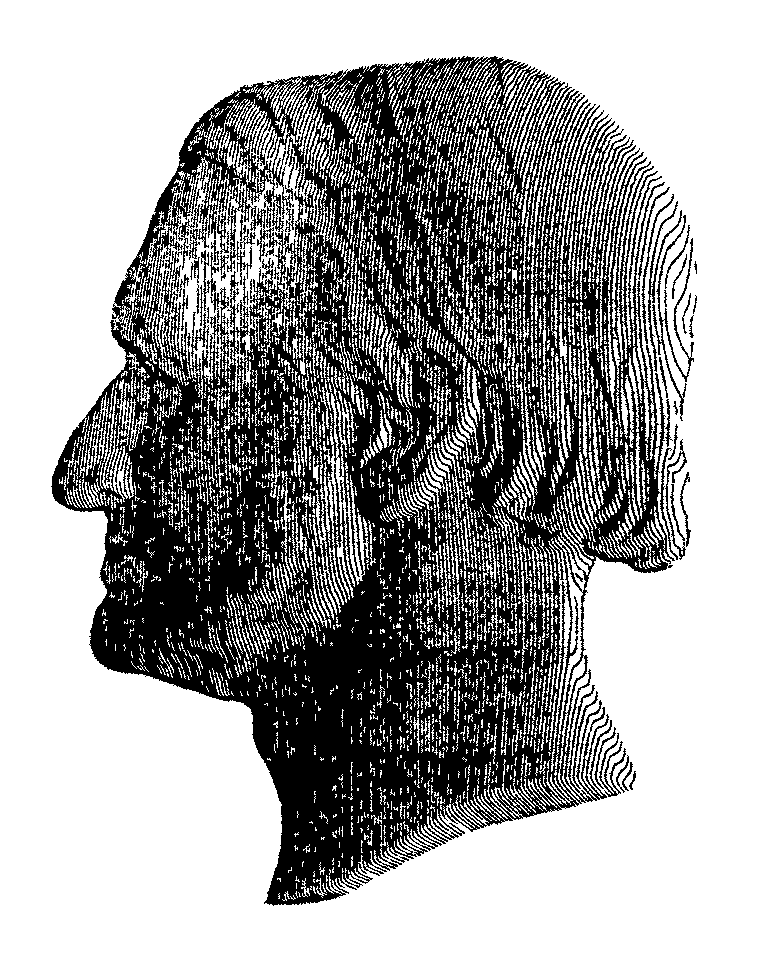
\includegraphics[width=1.65in]{assets/portrait_native004_complete.png}\\[2em]
\textbf{EDITED}\\[0.5em]
\textbf{BY THE}\\[0.5em]
\textbf{ROYAL SOCIETY OF SCIENCES}\\[0.5em]
\textbf{AT GÖTTINGEN}\\[1em]
\textbf{1866.}
\end{center}
\clearpage

\clearpage\thispagestyle{empty}\SourceLeaf{006}
\vspace*{1cm}
\begin{center}\small
\textbf{A NEW PROOF}\\[0.75em]
\textbf{OF THE THEOREM}\\[0.75em]
\textbf{THAT EVERY POLYNOMIAL}\\[0.5em]
\textbf{}\\[0.75em]
\textbf{IN ONE VARIABLE}\\[0.75em]
\textbf{CAN BE RESOLVED INTO REAL FACTORS}\\[0.75em]
\textbf{OF THE FIRST OR SECOND DEGREE}\\[1.5em]
\textbf{SUBMITTED FOR}\\[0.5em]
\textbf{THE HIGHEST HONOURS IN PHILOSOPHY}\\[0.5em]
\textbf{TO THE ILLUSTRIOUS FACULTY OF PHILOSOPHY}\\[0.75em]
\textbf{OF THE ACADEMIA JULIA CAROLINA}\\[1.5em]
\textbf{BY}\\[0.75em]
\textbf{CARL FRIEDRICH GAUSS}\\[1.5em]
\rule{0.65\linewidth}{0.4pt}\\[0.75em]
\textbf{HELMSTEDT}\\[0.5em]
\textbf{AT C. G. FLECKEISEN. MDCCLXXXXIX.}
\end{center}

\clearpage
